\providecommand{\main}{..}
\documentclass[\main/main.tex]{subfiles}

\begin{document}

\lesson{6}{15/10/20}
\section{Time-scale of convergence to equilibrium}
We have seen that MC is a stochastic process with memory oneb, which means that the update rule, which tells us how to find the probability of visiting state $j$ at time $t+1$ can be obtained with the sum of all the previous states $i$ and multipling it by the transition rate from $i$ to $j$:
\begin{align}
p_j(t+1) &=\sum_i W_{ji}p_i(t) \\
\Vec{p}(t+1) &=W\Vec{p}(t)
\end{align}
where $W_{ji}$ is stochastic matrix, which encodes the properties of the MC; if we find a solution of the eigenvalue problem for the stochastic matrix with eigenvalue $\lambda=1$, then this implies that the right eigenvector is a stationary distribution for the MC:
\begin{eqnarray}
W \Bar{w}^{(1)}=\Bar{w}^{(1)}\quad \implies \quad \Bar{w}^{(1)}=\text{stationary distribution}   
\end{eqnarray}

The theorems we have seen in the last lecture are: \\

\textbf{Theorem 1}: if a MC is irreducible and positive recurrent - which means that the average return time to any state $i$ is finite - then, upon these conditions 
\begin{eqnarray}
   \mean{T_i}<+\infty \implies \Bar{w}^{(1)} \,\text{\textit{{unique}} stationary distribution and }\, w_i^{(1)}=\frac{1}{\mean{T_i}}
\end{eqnarray}

\textbf{Theorem 2}: if a MC is irreducible, positive recurrent and aperiodic - meaning period (\ref{eq:period}) is equal to unity - then, upon these conditions we have convergence: for any choice of initial conditions we have that
\begin{eqnarray}
p_j(t)=\sum_i (W^{t})_{ji}p_i(0)\overset{t\to\infty}{\longrightarrow} w_i^{(1)}
\end{eqnarray}

Let's now characterize the time scale of convergence: let's study the MC in the case in which \textbf{Theorem 2} holds, whichmeans that we are dealing with a irreducible, positive recurrent and aperiodic MC (ergodic MC).
Using the Perron-Frobenius theorem, which states that
\begin{eqnarray}
\lambda^{(1)}=1>|\lambda^{(2)}|\geq|\lambda^{(3)}|\geq\dots
\end{eqnarray}
(the first eigenvalue is related to the the stationary distribution), we can use in general the set of right eigenvectors to express the probability vector as a linear combinations of all eigenvectors. The stochastic matrix is in general not symmetric and the eigenvalues can be complex numbers and we have right and left eigenvectors, where $k$ is referred to the corresponding eigenvalue and in this contex eigenvalues are ranked according to their norm:
\begin{eqnarray}
\Vec{p}(t)=\sum_k \alpha_k \Vec{w}^{(k)}, \quad \vec{w}^{(k)}\,\, \text{right eigenvectors} \\
\alpha_k(t)=\Vec{p}(t)\cdot\Vec{w}_l^{(k)}, \quad \Vec{w}_l^{(k)}\,\,\text{left eigenvectors}
\end{eqnarray}

We can express the probability vector at time $t$ as the action of the $t$ power of the stochastic matrix on the initial condition:
\begin{align}
    \Vec{p}(t) &=W^t \Vec{p}(0)=W^t[\sum_k \alpha_k(0)\Vec{w}^{(k)}] \\
    &=\sum_k \alpha_k(0) (\lambda^{(k)})^{t}\Vec{w}^{(k)}
\end{align}
From here we can see that the time dependence of the $\alpha_k$ coefficients can be expressed as:
\begin{eqnarray}
    \alpha_k(t)=\alpha_k(0)[\lambda^{(k)}]^t
\end{eqnarray}
In general eigenvalues are complex numbers, so:
\begin{eqnarray}
       \lambda^{(k)}=|\lambda^{(k)}|\exp(i \phi_k)
\end{eqnarray}

Now we are interested in evaluating the time dependence of these coefficients:
\begin{align}
    \alpha_k(t)&=\alpha_k(0)\exp(i t \phi_k)|\lambda^{(k)}|^t \\
    &=\alpha_k(0) \exp(it\phi_k)\exp(\frac{-t}{\tau_k})
\end{align}
where we introduced a characteristic time $\tau_k=-1/\ln(|\lambda_k|)>0$ since  $|\lambda_k|<1$ for $ (k\geq 2)$.
We are dealing then with an exponential decay in time of the $\alpha_k$ coefficient.

At this point we can isolate the term corresponding to the first eigenvalue, which corresponds to the stationary distribution, (and being stationary there is no time dependence in this term) and then we find:
\begin{eqnarray}
    \Vec{p}(t)=\alpha_1(0)\Vec{w}^{(1)}+\underbrace{\alpha_2(0)\exp(it\phi_2)\exp(-t/\tau_2)}_{\text{Leading term!}} +\dots
\end{eqnarray}

If we assume \textit{no degeneracy} the leading term is the second one, because $|\lambda^{(2)}|>|\lambda^{(k)}|$ and that means $\tau_2>\tau_k$. All other terms decay to zero exponentially and the term with the longest characteristic time is the one corresponding to the second largest normed eigenvalue.

To sum up, the characteristic time for convergence to stationarity is given by:
\begin{eqnarray}
  \boxed{  \tau_2=-\frac{1}{\ln{(|\lambda^{(2)}|)}}}
\end{eqnarray}
\section{Detailed balance}

In the infinite time limit we have discussed about \textit{stationary} conditions but to characterize \textit{equilibrium} we will need a stronger condition provided by detailed balance.

We will start by writing a master equation for MC. Let's write the update rule by adding and subtracting $p_i(t)$:
\begin{align}
        p_i(t+1) &=\sum_j W_{ij}p_j(t) +p_i(t)-p_i(t)\underbrace{\sum_{ij}W_{ji}}_{=1} \\
        &=p_i(t) + \sum_j [W_{ij}p_j(t) - W_{ji}p_i(t)]
\end{align}

and taking $p_i(t)$ to the left:
\begin{eqnarray}
   \underbrace{ p_i(t+1)-p_i(t)=\sum_{j\neq 1}[\underbrace{W_{ij}p_j}_{\text{gain term}}-\underbrace{W_{ji}p_i}_{\text{loss term}}]}_{\text{Master Equation}}
\end{eqnarray}
where the gain term is the sum over all possible previous states, while in the loss term we sum all over the possible arrival states.

Now it is immediate to see that the stationarity condition (which means $p_i(t+1)-p_i(t)=0$) is related to:
\begin{eqnarray}
   \text{Stationarity condition}\quad \iff \quad \sum_{j\neq 1}[{W_{ij}p_j}-{W_{ji}p_i}]=0 \,\, \forall \, i
\end{eqnarray}
but we can have a stronger condition, called \textbf{detailed balance}, where each single summands in the above term must be zero:
\begin{eqnarray}
   \text{Detailed balance}\qquad \iff \qquad {W_{ij}p_j}={W_{ji}p_i} \,\, \forall \, i\neq j
   \label{eq:db}
\end{eqnarray}

Obviously detailed balance implies stationarity but not the other way.

\subsection{Connection between detailed balance and reversibility}
A MC for which a detailed balance is satisfied is called \textbf{\textit{reversible MC}} and reversibility is connected to \textit{time reversal invariance}: thermodinamic equilibrium is connected to microscopic reversibility. \\

When we talk about time reversal invariance essentially we say that the probability of a forward trajectory is equal to the probability of a backwards trajectory using the same dynamical rule i.e. the same stochastic matrix.

Let's consider a forward trajectory: we divide the time in $t_i=\{t_1,t_2, \dots, t_n\}$ and we have a sequence of corresponding states $\{s_{i_0}, s_{i_1},s_{i_2},\dots, s_{i_n}\}$. What is the probability of observing such trajectory for a given MC/stochastic matrix? \\

we want to write the probability that we observe the state $s_{i_n}$ at time $n$ and so on:
\begin{eqnarray}
   p (x(n)=s_{i_n}; x(n-1)=s_{i_{n-1}}; \dots; x(1)=s_{i_1}; x(0)=s_{i_0})
\end{eqnarray}

How we write this? For the initial state we have to chose an initial condition: we will chose the stationary distribution $p_{i_0}$ for which detailed balance holds:
\begin{eqnarray}
  {p_{i_0}}\cdot W_{i_1, i_0} \cdot W_{i_2,i_1} \cdot \,\,\dots \,\, \cdot W_{i_n,i_{n-1}} =
  \label{eq:ft}
\end{eqnarray}

Th point is now that we can use detailed balance and we can rewrite ${p_{i_0}}\cdot W_{i_1, i_0}$ switching the indices of the stochastic matrix and getting $W_{i_0, i_1}\cdot{p_{i_1}}$ using (\ref{eq:db}). 
We can do this subsequently for all terms considering now  $\{{p_{i_1}}\cdot W_{i_2, i_1} \to W_{i_1, i_2}\cdot {p_{i_2}}\}$ and so on.

In the end we will obtain the following expression for the probability of a forward trajectory (\ref{eq:ft}):
\begin{align}
    = W_{i_0, i_1} \cdot W_{i_1, i_2} \cdot\,\, \dots\,\, \cdot W_{i_{n-1}, i_n} \cdot p_{i_n}
\end{align}
and this is just the expression for the backward trajectory, because now we can start from the right side of this product and it is just the probability of starting in the $i_n$ state and then going to the $i_{n-1}$ one and so one until we get to state $i_{0}$:
\begin{eqnarray}
  \underbrace{p (x(n)=s_{i_0}; x(1)=s_{i_{1}}; \dots; x(0)=s_{i_n})}_{\text{Probability of backward trajectory}}
\end{eqnarray}
This is crucial because it shows the connection between detailed balance and microscopic reversibility.

\begin{center}
    \textbf{{Detailed balance $\Longleftrightarrow$ equilibrium (microscopic reversibility)}} \\
    stronger condition than just stationarity
\end{center}

\subsection{MC example: Random Walk on a ring}
We will see now an example of a Random walk on a ring in one dimension: we are dealing with $N$ states (finite space states) and our dynamical rule is such that for a given state $i$ we can go either on the previous state $i-1$ with probability $r-1$ or to the next state $i+1$ and this may happen with probability $r$. the schematics of our example is represented in Figure (\ref{fig:ring_rw}). In this problem state $N+1$ is equal to state 1, we are using PBC.
%\par\medskip
\begin{figure}[ht]
    \centering
    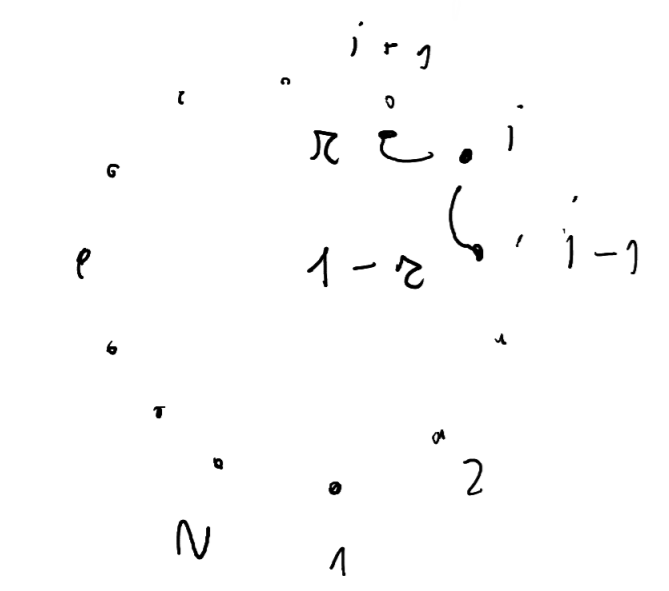
\includegraphics[width=0.4\linewidth]{Lectures/Images/ring_rw.png}
    \caption{Random Walk on a ring using with states, forward probability $r$ and backwards probability $r-1$.}
    \label{fig:ring_rw}
\end{figure}

\begin{numcases}{\text{More formally:\,\,}}
  W_{i_{i+1}, i_i}=r  \\
  W_{i_{i-1}, i_i}=1-r & \\
  W_{i.j}=0 & {otherwise}
\end{numcases}

An important observation is that the diagonal elements $W_{i,i}=0$ so is not possible to remain in the same state: we have either go the the right or to the left.Obviously $0\leq r \leq 1$ because it's a probability.

If we chose:
\begin{itemize}
    \item $r=\frac{1}{2} \longrightarrow$: \textbf{symmetric (unbiased) random walk};
    \item $r\neq\frac{1}{2} \longrightarrow$: \textbf{asymmetric (biased) random walk}.
\end{itemize}

We can explicitly visualize our stochastic matrix associated to a random walk on a ring:
\begin{center}
\[
W =
\begin{pmatrix}
0 & 1-r & 0 & 0 & 0 & \dots &r\\
r & 0 & 1-r & 0 & 0&  & 0 \\
0 & r & 0 & 1-r & 0 &  & \vdots \\
\vdots & 0 & \ddots & \ddots & 1-r & & \vdots\\
\vdots & &\ddots & \ddots & \ddots & \ddots &\vdots \\
\vdots & & & \ddots &\ddots & \ddots& 1-r \\
1-r & \dots & \dots& \dots& 0 & r & 0
\end{pmatrix}
\]
\end{center}

The last entry on the first row is $r$ due to PBC. \\

Let's now have a look to the stochastic update rule: 
\begin{eqnarray}
  p_i(t+1)=(1-r)p_{i+1}(t)+r\, p_{i-1}(t)
  \label{eq:1}
\end{eqnarray}
We are interested in the stationary distribution, $\hat{p}_i$, which has to satisfy equation (\ref{eq:1}) without any dependence in time:
\begin{align}
    \hat{p}_i=(1-r)\hat{p}_i + r\, \hat{p}_i
\end{align}
The obvious solution is the one with constant probability $\hat{p}_i=\frac{1}{N}$: all the vector components are equal each other and each component is $N^{-1}$ for normalization, because we want that the probability vector is normalized such that $\sum_{i=1}^N \hat{p}_i=1$.

Obviously, considering this solution, the stationarity condition holds $\forall \,i$. \\

Now the issue is \textit{uniqueness} and \textit{convergence}: let's have a look to the whole spectrum of the stochastic matrix $W$.

Starting from the eigenvalue equation:
\begin{eqnarray}
  W\Bar{w}=\lambda\Bar{w}
\end{eqnarray}
 In our specific example the eigenvalue problem becomes (using $k$ to label the states on the ring\footnote{We will not use $i$ anymore because we will deal with complex eigenvalues.}):
 \begin{eqnarray}
   (1-r)w_{k+1} + r\, w_{k-1}=\lambda w_k
   \label{eq:eGV}
 \end{eqnarray}
 \textit{Ansatz for the solution} that will allow us to find the solution: let's rewrite the $k$ component of the eigenvector $w$ as follows:
 \begin{align}
     w_k:=\omega^k
     \label{eq:ansatz}
 \end{align}
 
 where $\omega$ is determined by PBC. Using this ansatz we impose that:
 \begin{eqnarray}
   w_{N+1}=w_1
 \end{eqnarray}
 and this conditions tells us that
 \begin{eqnarray}
   \boxed{\omega^N=1}
 \end{eqnarray}
 We have $N$ solutions of this equation and we need to deal with complex numbers:
 \begin{align}
     \omega_j=\exp(\frac{2\pi i}{N}j)
     \label{eq:omega}
 \end{align}
 where $i$ is the imaginary unite, while $j$ is an integer going from zero to $N-1$: $j=\{0,1,\dots,N-1\}$. These are all the possible solutions to the condition implied by the PBC on the ring, so now $j$ labels eigenvalues and eigenvectors. \\
 
 Let's now use Eq. (\ref{eq:eGV}): if we substitute the ansatz for the eigenvector component we can see that the $j^{th}$ eigenvalue (remember that $j$ labels different eigenvalues) can be written in this way:
 \begin{align}
     \lambda_j=(1-r)\,\omega_j + r \frac{1}{\omega_j}=
 \end{align}
 then, using (\ref{eq:omega}) and the Euler equation to express the exponential of the imaginary number as a sum of sin and cos functions:
\begin{align}
    = \cos(\frac{2\pi j}{N}) + i(1-2r)\sin(\frac{2\pi j}{N})
\end{align} 

Let's now have a look to what happens in the symmetric and asymmetric case

\paragraph{Symmetric case, $r=1/2$:}

we can see in this case that, in the eigenvalues, the imaginary part vanishes: the eigenvalues are always real numbers:
\begin{eqnarray}
  \lambda_j=\cos(\frac{2\pi j}{N}) \in \mathbb{R}
\end{eqnarray}
Considering the transition rates then 
\begin{eqnarray}
  r=\frac{1}{2} \qquad \implies \qquad W_{ij}=W_{ji}
\end{eqnarray}
The fact that we get real eigenvalues is not surprising: in fact the stochastic transition matrix is symmetric in this case.

\paragraph{Asymmetric case, $r\neq1/2$:}
Let's start by considering the eigenvalue $\lambda_0$\footnote{In this passage we need to be careful: the labeling of eigenvalues that we are using now depends on the way we enforce the PBC and is not consistent with the ranking used at the beginning of this section.}. If $j=0$ then:
\begin{eqnarray}
  \lambda_0 = 1
\end{eqnarray}
and the eigenvectors have in general components of this type (using ansatz (\ref{eq:ansatz})):
\begin{eqnarray}
 (1,\omega_j,\omega_j^2,\dots,\omega_j^N)
\end{eqnarray}

In the case with $j=0$ the corresponding eigenvector\footnote{I'm not considering normalization in the way we wrote this eigenvector.} is:
\begin{eqnarray}
    \Bar{w}^{(0)}=(1,1,\dots,1)
\end{eqnarray}
because $\omega_0=1$, as we can see from Eq. (\ref{eq:omega}). 

In the asymmetric case the imaginary part is non vanishing for $j\neq0$. In general $\lambda_j\, \in\, \mathbb{C}$ for $j>1$ and as we can see $W_{ij}\neq W_{ji}$.

The interesting point of this example is:
\begin{itemize}
    \item in the symmetric case the detailed balance holds because (\ref{eq:db}) is verified but we need to remember that the stationary distribution is the constant one and the transition matrix is symmetric and we have \textit{no currents in the system}: the fact that random walk is unbiased implies that \textit{the average velocity of the random walker is zero.}
    \begin{center}
        equilibrium and D.B. holds $\implies$ no currents in the system
    \end{center}
    \item in the asymmetric case we don't have detailed balance because $p_i{W_{
    ji}}\neq{p_j W_{ij}}$: the stationary distribution $\hat{p}_i=1/N$ is the same in both cases but the stochastic matrix isn't symmetric anymore. A current is flowing in the system (the random walker has a drift velocity).
\end{itemize}

This is a specific example in which we have \textit{stationarity} but \textit{no equilibrium}. If we compute explicitly the average velocity: 
\begin{eqnarray}
    v=\underbrace{(+1)\,r}_{\text{Moving to R}} +\,\, \underbrace{(-1)\,(1-r)}_{\text{Moving to L}}=
\end{eqnarray}

\begin{numcases}{= 2r-1 = \,\,}
  >0 & $r>\frac{1}{2}$\\
  =0 & $r=\frac{1}{2}$ \\
  <0 & $r=\frac{1}{2}$
\end{numcases}

\paragraph{Problems with convergence:} this example provides a case in which the assumptions needed to prove convergence in Theorem 2 are not satisfied if $N$ is even. 

In this case we can realize that we have periodicity with period 2: let's say we start at state 1, then on the next step we either go the the R or to the L. At even times we will always be at odd states and at odd times we will always be at even states \textit{and this is true for any given time}.

Since the hypotheses of Theorem 2 are not satisfied we expect no convergence and what happens as a matter of fact is that:
\begin{eqnarray}
    p_i(t)\underset{t\to \infty}{\longrightarrow}\frac{1}{N} \,\, (=\hat{p}_i) \quad \text{does not hold for all initial conditions}
\end{eqnarray}

We can take as an example the one in which the initial condition is localized in the first state:
\begin{align}
    p_i(0)=\delta_{i,1}
\end{align}
and the fact that we don't see convergence is actually related to the presence of a second eigenvalue with norm equal to one and so the time scale convergence goes up to infinity.
In fact, if $j=N/2$
\begin{eqnarray}
    \lambda_{N/2}=-1 \to \bar{w}^{(N/2)}=(+1,-1,+1,-1,\dots)
\end{eqnarray}
Nevertheless, even if we are in a situation in which we don't have formal convergence in the sense just discussed, we have a sort of \textit{weak convergence}. In fact, considering the limit:
\begin{align}
    \lim_{t\to\infty}\frac{1}{t}\sum_{r_i=1}^{t}p_j(r_i)=\frac{1}{N}
\end{align}
it converges to the stationary distribution. In this way we average over the odd and even times and we recover the correct stationary distribution.




 
\end{document}